\documentclass[12pt,letterpaper]{article}

\usepackage[brazilian]{babel}
\usepackage[utf8]{inputenc}
\usepackage[T1]{fontenc}

\usepackage{fullpage}
\usepackage{cancel}
\usepackage[top=2cm, bottom=4.5cm, left=2.5cm, right=2.5cm]{geometry}
\usepackage{amsmath,amsthm,amsfonts,amssymb,amscd}
\usepackage{lastpage}
\usepackage{enumerate}
\usepackage{fancyhdr}
\usepackage{mathrsfs}
\usepackage{xcolor}
\usepackage{graphicx}
\usepackage{listings}
\usepackage{hyperref}

\hypersetup{%
	colorlinks=true,
	linkcolor=blue,
	linkbordercolor={0 0 1}
}

\setlength{\parindent}{0.0in}
\setlength{\parskip}{0.05in}

% Edit these as appropriate
\newcommand\course{Rener Oliveira}
\newcommand\lcur{\mathcal{L}}
\newcommand{\real}{\mathbb{R}}
\newcommand{\rr}{\mathbb{R}^2}
\newcommand{\rn}{\mathbb{R}^n}
\newcommand{\linesep}{{\color{black} \rule{\linewidth}{0.5mm} }}
\newcommand{\rpos}{\mathbb{R}_{>0}}
\newcommand{\ex}[1]{\textcolor{blue}{\textbf{Exercício #1}}}
\newcommand{\sol}[1]{\textbf{Solução #1}}
\newcommand{\blue}[1]{{\color{blue}{#1}}}
\newcommand{\bd}[1]{\boldsymbol{#1}}
\pagestyle{fancyplain}
\headheight 35pt        
\chead{\textbf{\Large Lista 4 \\ Curvas e Superfícies}}
\rhead{\small{\course \\ \today}}
\lfoot{}
\cfoot{}
\rfoot{\small\thepage}
\headsep 1.5em

\begin{document}
	\begin{enumerate}
		
		\item [\ex{1}] \textcolor{blue}{Verifique se as seguintes curvas são 2-regulares:}
		\begin{enumerate}[(a)]
			\blue{
			\item $\alpha(t)=(t,t^2,t^3),t\in\real$
			}
			
		Usaremos a definição de \cite{ronaldo}, para curvas 2-regulares, que diz que a curva precisa ser regular e com curvatura estritamente positiva.
		
		Veja que $\alpha'(t)=(1,2t,3t^2)$ que é diferente do vetor nulo, para todo $t$ real por conta da primeira componente  constante igual a $1$. Logo $\alpha$ é regular. Pelo item 7, a curvatura é $\kappa_\alpha(t)=2\sqrt{\dfrac{1+9t^2+9t^4}{(1+4t^2+9t^4)^3}}$, que só seria nula no caso $1+9t^2+9t^4=0$ o que não ocorre, dado que $(9t^2+9t^4)\geq0$ e $1>0$. Logo $\alpha$ é 2-regular.
		
		
		
		\blue{
			\item $\alpha(t)=(t,t^2+2,t^3+t),t\in\real$}
		
		Temos $\alpha'(t)=(1,2t,3t^2+1)$ e $\alpha''(t)=(0,2,6t)$, a velocidade é não-nula pelo termo constante o que faz $\alpha$ ser regular. Usaremos a aceleração no cálculo da curvatura:
		
		\begin{align*}
			\kappa_{\alpha}(t)&=\dfrac{||\alpha''(t)\times\alpha'(t)||}{||\alpha'(t)||^3}\\
			&=\dfrac{||(0,2,6t)\times(1,2t,3t^2+1)||}{||(1,2t,3t^2+1)||^3}\\
			&=\dfrac{||(2-6t^2,6t,-2)||}{(1+4t^2+(3t^2+1)^2)^{3/2}}\\
		\end{align*}
		
		Para evitar contas, dado que queremos analisar se a curvatura é nula ou não, vamos olhar somente o numerador:
		
		\begin{align*}
			||(2-6t^2,6t,-2)||&=\sqrt{(2-6t^2)^2+36t^2+4}\\
			&=\sqrt{4-24t^2+36t^4+36t^2+4}\\
			&=\sqrt{8+12t^2+36t^4}\\
			&\geq0\text{ }\forall t \in \real,\text{ pois } (12t^2+36t^4)\geq0\text{ e } 8>0
		\end{align*}
		
		Com isso, concluímos que $\alpha$ é 2-regular.
	\end{enumerate}

	\item[\ex{2}] \textcolor{blue}{Prove que a aplicação $\alpha(t) = (1 +\cos(t),\sin(t),2\sin(t/2)),t\in\real$, é uma curva regular cujo traço está contido na interseção do cilindro $C= (x,y,z)\in\real^3; ~(x-1)^2+y^2= 1$ e da esfera $S= (x,y,z)\in\real^3;~x^2+y^2+z^2= 4$. Desenhe a curva $\alpha$, o cilindro $C$ e a esfera $S$ em ambiente computacional}
	
	\item[\sol{2}] A duas primeiras coordenadas da velocidade, a menos de sinal, são $\sin (t)$ e $\cos(t)$ que já foi provado no início da \href{https://github.com/reneroliveira/Curves_and_Surfaces/blob/main/lists/list3.pdf}{Lista 3} que não serão ao mesmo tempo. A terceira componente é, à menos de constantes $\cos(t/2)$. É fácil ver que ela não zera quando $\cos(t)=0$; O único problema seria com ângulos $t=\pi+2k\pi$, onde $\sin(t)=\cos(t/2)=0$, mas neste caso a componente $\cos(t)\neq0$. Podemos então assegurar que as componentes não se anulam ao memso tempo, comprovando a regularidade da curva.
	
	Na Figura \ref{ex2}, segue uma captura do conteúdo do arquivo \href{https://github.com/reneroliveira/Curves_and_Surfaces/blob/main/ggb_files/L4_ex2.ggb}{L4\_ex2.ggb}. Como podemos ver, de fato o traço da curva está contido na interseção das duas superfícies, o que termina nossa demonstração.
	\begin{figure}[!htb]
		\centering
		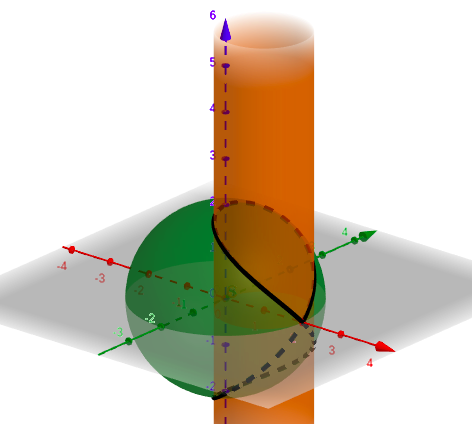
\includegraphics[scale=0.7]{../images/L4_ex2.png}
		\caption{Interseção de cilindro e esfera}
		\label{ex2}
	\end{figure}

	Brindadeiras a parte, vamos dar a prova formal de que o traço está na interseção. O cilindro $C$ é o lugar geométrico do $\real^3$ dos pontos equidistantes (distância = 1) do eixo central, que, no caso, é dado pela reta que passa por $(1,0,0)$ paralela ao eixo $z$.
	
	A esfera $S$ é o lugar geométrico do espaço dos pontos que distam 2 unidades da origem $O=(0,0,0)$.
	
	Para provar provar que $\alpha(\real)\subset C\cap S$, basta provar que 
	
	$$||\alpha(t)-(1,0,0)||_*=1,\text{ e }$$
	$$||\alpha(t)-O||=2~\forall t \in \real,$$
	
	onde $||.||_*$ é um operador de norma que leva em conta somente as duas primeiras componentes dados que estamos calculando distância à uma reta paralela ao eixo $z$.
	Fazendo os cálculos, temos então:
	
	\begin{align*}
		||\alpha(t)-(1,0,0)||_*&=||(1 +\cos(t),\sin(t),2\sin(t/2))-(1,0,0)||_*\\
		&=||(\cos(t),\sin(t),2\sin(t/2))||_*\\
		&=\sqrt{\cos^2(t)+\sin^2(t)}\\
		&=\sqrt{1}=1
	\end{align*}
	
	Provando então que o traço de $\alpha$ pertence a $C$.
	
	\begin{align*}
		||\alpha(t)-O||&=||(1 +\cos(t),\sin(t),2\sin(t/2))||\\
		&=\sqrt{1+2\cos(t)+\cos^2(t)+\sin^2(t)+4\sin^2(t/2)}\\
		&=\sqrt{2+2\cos(t)+4\cdot\dfrac{1-\cos(t)}2}\\
		&=\sqrt{2+\cancel{2\cos(t)}+2-\cancel{2\cos(t)}}\\
		&=\sqrt{4}=2
	\end{align*}

	Como queríamos demonstrar.
	\item[\ex{3}] \textcolor{blue}{Obtenha uma reparametrização por comprimento de arco da curva }
	\blue{
	$$\alpha(t)=(e^t\cos(t),e^t\sin(t),e^t),~t\in\real$$}
	\item[\sol{3}] Encontrando a função comprimento de arco:
	
	\begin{align*}
		\lcur(t)&=\int_{t_0}^{t}||\alpha'(u)||du\\
		&=\int_{t_0}^{t}||e^u(-\sin u,\cos u,1)||du\\
		&=\int_{t_0}^{t}e^u(\sin^2u+\cos^2u+1)^{1/2}du\\
		&=\sqrt2\int_{t_0}^{t}e^udu\\
		&=\sqrt2(e^t-e^{t_0})
	\end{align*}
		
		Tomando os devidos cuidados com os domínios e imagens, podemos inverter a função comprimeiro de arco, fixando  gerando $\lcur^{-1}(t)=\ln\left(\dfrac{t}{\sqrt2}+e^{t_0}\right)$
		
		Assim, tomando $s_t=\dfrac{t}{\sqrt2}+e^{t_0}$ a reparametrização por comprimeiro de arco será:
		
		\begin{align*}
			\alpha(\lcur^{-1}(t))&=s_t\left(\cos\left(s_t\right),\sin\left(s_t\right),1\right),
		\end{align*}
	
	Onde está definida para valores de $t$ na qual $\dfrac{t}{\sqrt2}+e^{t_0}>0\Rightarrow t>-e^{t_0}\sqrt2$.
	
	\item[\ex{4}]\textcolor{blue}{Seja $\alpha:I\to\real^3$ uma curva regular. Prove que $||\alpha'(t)||$ é constante se, e só se,$\forall t \in I, ~\alpha''(t)$ é ortogonal a $\alpha'(t)$. Em particular, mostre que $||\alpha'(t)||$ é constante para a hélice circular $\alpha(t) = (a\cos(t),a\sin(t),bt),t\in\real$.}
	
	\item[\sol{4}] Como a curva é regular $||\alpha'(t)||>0, ~\forall t\in I$. Dada uma constante $c\in\rpos$, temos então:
	
	\begin{align*}
		||\alpha'(t)||=c&\Leftrightarrow||\alpha'(t)||^2=c^2\\
		&\Leftrightarrow \dfrac{d}{dt}\langle\alpha',\alpha'\rangle=0\\
		&\Leftrightarrow\langle\alpha',\alpha''\rangle+\langle\alpha'',\alpha'\rangle=0\\
		&\Leftrightarrow2\langle\alpha',\alpha''\rangle=0\\
		&¨\Leftrightarrow\langle\alpha',\alpha''\rangle=0
	\end{align*}

	Logo $\alpha''(t)$ é ortogonal a $\alpha'(t)$.
	
	Para o caso particular da hélice, temos:
	
	\begin{align*}
		||\alpha'(t)||&=||(a\cos(t),a\sin(t),bt)'||\\
		&=||(-a\sin(t),a\cos(t),b)||\\
		&=\sqrt{a^2(\sin^2(t)+\cos^2(t))+b^2}\\
		&=\sqrt{a^2+b^2},
	\end{align*}
	
	que é constante, pois $a$ e $b$ são arbitrários, mas fixos.

	\item[\ex{7}] \textcolor{blue}{Calcule a curvatura e a torção das seguintes curvas:}
		\begin{enumerate}[(a)]
			\blue{
			\item $\alpha(t)=(t,t^2,t^3),t\in\real$}
				\begin{align*}
					\kappa_{\alpha}(t)&=\dfrac{||\alpha''(t)\times\alpha'(t)||}{||\alpha'(t)||^3}
					=\dfrac{||(0,2,6t)\times(1,2t,3t^2)||}{||(1,2t,3t^2)||^3}\\
					&=\dfrac{||(-6 t^2, 6 t, -2)||}{(1+4t^2+9t^4)^{3/2}}
					=\dfrac{2||(-3t^2,3t,-1)||}{(1+4t^2+9t^4)^{3/2}}\\
					&=\dfrac{2(1+9t^2+9t^4)^{1/2}}{(1+4t^2+9t^4)^{3/2}}\\
					&=2\sqrt{\dfrac{1+9t^2+9t^4}{(1+4t^2+9t^4)^3}}
				\end{align*}
			
			
			
			\begin{align*}
				\tau_\alpha(t)&=\dfrac{\langle(\alpha'(t)\times\alpha''(t)),\alpha'''(t)\rangle}{||\alpha'(t)\times\alpha''(t)||^2}\\
				&=\dfrac{\langle(6 t^2, -6 t, 2),(0,0,6)\rangle}{||(6 t^2, -6 t, 2)||^2}\\
				&=\dfrac{12}{36t^4+36t^2+4}\\
				&=\dfrac{3}{9t^4+9t^2+1}
			\end{align*}
		
		\blue{\item $\beta(t)=(\cos t,\sin t,t),t\in\real$}
		
		Como $||\beta'(t)||=||(-\sin t,\cos t,1)||=\sqrt2$ a curva $\beta$ não é unit-speed, podemos reparametrizar por comprimento de arco, trnasformá-la em unit-speed e calcular a curvatura e torção a partir daí. 
		
		É fácil ver que fazendo $t_0=0$, $\lcur_\beta(t)=\sqrt2t$, logo $\lcur^{-1}_\beta(t)=t/\sqrt2$, e a cruva reparametrizada será:
		
		$$\beta(t)=(\cos(t/\sqrt2),\sin(t/\sqrt2),t/\sqrt2)$$
		\begin{align*}
			\kappa_{\beta}(t)&=||\beta''(t)||\\
			&=\dfrac{1}{\sqrt2}||(-\sin (t/\sqrt2),\cos (t/\sqrt2),1/\sqrt2)'||\\
			&=\dfrac{1}{2}||(-\cos (t/\sqrt2),-\sin (t/\sqrt2),0)||\\
			&=\dfrac{1}{2}\sqrt{\sin^2(t/\sqrt2)+\cos^2(t/\sqrt2)}\\
			&=\dfrac{1}{2}
		\end{align*}
		
		Para a torção, vamos determinar os vetores tangente (T), normal (N) e binormal (B), do Triedro de Frenet, e calcular torção como a $\tau(s)$ tal que $B'(s)=\tau(s)N(s)$.
		
		\begin{align*}
			T(s)&=\dfrac{1}{\sqrt2}(-\sin (s/\sqrt2),\cos (s/\sqrt2),1)\\
			N(s)&=(-\cos (s/\sqrt2),-\sin (s/\sqrt2),0)\\
			B(s)&=T(s)\times N(s)\\&=\dfrac{1}{\sqrt2}(\sin(s/\sqrt2),-\cos(s/\sqrt2),1)
		\end{align*}
		\end{enumerate}
	\item[\ex{11}]\textcolor{blue}{Verifique que o vetor binormal de uma hélice circular forma um ângulo constante como eixo do cilindro sobre o qual está a hélice. Ilustre o fato em ambiente computacional.}
	
	\item[\sol{11}] Dada a hélice circular $\alpha(t)=(a\cos(t),a\sin(t),bt)$ com um cálulo similar ao que foi feito na questão 7, que está detalhado em \cite{ronaldo}, obtemos a seguinte reparametrização por comprimento de arco, considerando $\ell=\sqrt{a^2+b^2}$,
	
	\begin{align*}
		\alpha(s)&=\left(a\cos\left(s/\ell\right),a\sin\left(s/\ell\right),bs/{\ell}\right)
	\end{align*}
	
	Assim a curva fica \textit{unit-speed} e teremos:
	
	\begin{align*}
		T(s)=\alpha'(s)=\dfrac1\ell(-a\sin(s/\ell),a\cos(s/\ell),b)
	\end{align*}
	`
	O vetor normal $N(s)$ é o unitário da aceleração. 
	
	\begin{align*}
		\alpha''(s)&=\dfrac{1}{\ell^2}(-a\cos(s/\ell),-a\sin(s/\ell),0)\\
		||\alpha''(s)||&=\dfrac{1}{\ell^2}\sqrt{a^2}=\dfrac{|a|}{\ell^2}\\
		N(s)&=\dfrac{\alpha''(s)}{||\alpha''(s)||}=-\dfrac{a}{|a|}(\cos(s/\ell),\sin(s/\ell),0)
	\end{align*}
	
	Assim, o binormal será:
	
	\begin{align*}
		B(s)&=T(s)\times N(s)\\
		&=-\dfrac{a}{\ell|a|}(-a\sin(s/\ell),a\cos(s/\ell),b)\times(\cos(s/\ell),\sin(s/\ell),0)\\
		&=-\dfrac{a}{\ell|a|}(-b\sin(s/\ell),b\cos(s/\ell),-a)
	\end{align*}

	Tal hélice está no cilindro de eixo $z$, queremos provar que o ângulo entre o binormal e tals eixo é constante. Tomemos o vetor $\vec v=(0,0,1)$, vamos então calcular o cosseno entre $B$ e $v$ e mostrar que é constante.
	
	\begin{align*}
		\cos(B(s),\vec v)&=\dfrac{\langle B(s),\vec v\rangle}{||B(s)||\cdot||\vec v||}\\
		&=\dfrac{a^2/\ell|a|}{||B(s)}\\
		&=\dfrac{a^2/\ell|a|}{a/\ell|a|\cdot ||(-b\sin(s/\ell),b\cos(s/\ell),-a)||}\\
		&=\dfrac{a^2/\ell|a|}{a/\ell|a|\cdot \sqrt{a^2+b^2}}\\
		&=\dfrac{a}{\ell},
	\end{align*}
	que é contante, como queríamos demonstrar.
	\end{enumerate}
	\newpage

% \addcontentsline{toc}{section}{Referências}
\bibliographystyle{plain}
\bibliography{refs}
\end{document}